\documentclass[conference,twocolumn]{IEEEtran}
\IEEEoverridecommandlockouts
% The preceding line is only needed to identify funding in the first footnote. If that is unneeded, please comment it out.
\usepackage{cite}
\usepackage{amsmath,amssymb,amsfonts}
\usepackage{algorithmic}
\usepackage{graphicx}
\usepackage{textcomp}
\usepackage{xcolor}

\usepackage[acronym]{glossaries}
\usepackage{tikz}
\usetikzlibrary{positioning, shadows, fit}
\usepackage{booktabs}
\usepackage{url}
\usepackage{multirow}
\usepackage{tabularx}
\usepackage{dblfloatfix}

% Acronyms  
\newacronym{ai}{AI}{artificial intelligence}
\newacronym{ml}{ML}{machine learning}
\newacronym{automl}{AutoML}{automated machine learning}
\newacronym{hcai}{HCAI}{human-centered artificial intelligence}
\newacronym{hgml}{HGML}{human-guided machine learning}
\newacronym{gui}{GUI}{Graphical User Interface}
\newacronym{ui}{UI}{User Interface}
\newacronym{dl}{DL}{Deep Learning}
\newacronym{hci}{HCI}{Human-Computer Interaction}  
\newacronym{auc_roc}{AUC-ROC}{Area Under the Receiver Operating Characteristic Curve}  
\newacronym{mae}{MAE}{Mean Absolute Error}  
\newacronym{rmse}{RMSE}{Root Mean Squared Error}  
\newacronym{shap}{SHAP}{SHapley Additive exPlanations}  
\newacronym{lime}{LIME}{Local Interpretable Model-agnostic Explanations}  
\newacronym{xai}{XAI}{Explainable Artificial Intelligence}
\newacronym{crp}{CRP}{clinical research professional}
\newacronym{hamelin}{HAMELIN}{Human-guided Automated Machine Learning for Clinical Studies}
\newacronym{icu}{ICU}{intensive care unit}
\newacronym{llm}{LLM}{large language model}


\def\BibTeX{{\rm B\kern-.05em{\sc i\kern-.025em b}\kern-.08em
    T\kern-.1667em\lower.7ex\hbox{E}\kern-.125emX}}
\begin{document}

\title{Towards a Human-Guided AutoML Application for Democratizing Predictive Modeling\\ in Clinical Research\\
\thanks{This work has been supported by grant  PID2023-146243OB-I00 funded by MICIU/AEI/10.13039/501100011033 and by ``ERDF/EU''.}
}

\author{\IEEEauthorblockN{Diego Garc\'ia-Prieto}
\IEEEauthorblockA{\textit{Dept. of Mathematics, Statistics and Computer Science} \\
\textit{University of Cantabria}\\
Santander, Spain \\
diego.garciaprieto@unican.es}
\and
\IEEEauthorblockN{Camilo Palazuelos}
\IEEEauthorblockA{\textit{Dept. of Mathematics, Statistics and Computer Science} \\
\textit{University of Cantabria}\\
Santander, Spain \\
camilo.palazuelos@unican.es}
\and
\IEEEauthorblockN{Rafael Duque}
\IEEEauthorblockA{\textit{Dept. of Mathematics, Statistics and Computer Science} \\
\textit{University of Cantabria}\\
Santander, Spain \\
rafael.duque@unican.es}
\and
\IEEEauthorblockN{Luc\'ia Lav\'in-Alconero}
\IEEEauthorblockA{\textit{Clinical Trials Agency Valdecilla-IDIVAL} \\
\textit{Marqu\'es de Valdecilla University Hospital}\\
Santander, Spain \\
lucia.lavin@idival.org}
}

\maketitle

\begin{abstract}
Clinical research faces a notable gap between the advanced capabilities of machine learning and their practical adoption by non-technical researchers. In addition, existing AutoML tools tend to treat clinical data as generic datasets, thereby ignoring the methodological particularities of patient registries, observational studies and clinical trials. To address these limitations, we present HAMELIN, an AutoML application under active development that aims to bridge this gap through a protocol-aware interface aligned with the principles of human-guided machine learning. In this way, HAMELIN enables researchers to build predictive models without requiring coding skills while incorporating their domain knowledge at every stage of the modeling process. The system was designed through iterative collaboration with clinical research professionals using real clinical protocols. This paper describes its design principles, architecture and implementation, and evaluates its alignment with human-guided machine learning criteria.
\end{abstract}

\begin{IEEEkeywords}
Automated Machine Learning, Human-Guided Machine Learning, Healthcare, Clinical Research, Protocol-Aware Systems
\end{IEEEkeywords}


\section{Introduction}
\label{sec:introduction}

The rapid integration of \gls{ai} into medicine has opened new opportunities for clinical research, enabling the development of predictive models that can support diagnosis, prognosis and treatment decisions \cite{sirocchi2024medical}. Among the most promising developments in this area is \gls{automl}, which automates complex tasks such as feature engineering, algorithm selection and hyperparameter optimization, enabling users without extensive programming expertise to build predictive models \cite{karmaker2021automl}. By reducing the technical barrier to entry, \gls{automl} platforms have the potential to democratize predictive modeling across a wide range of domains, including clinical research.

Building on these advances, \gls{hgml} \cite{gil2019towards} proposes a more 
collaborative paradigm: rather than fully automating the modeling process, it emphasizes integrating human expertise throughout the \gls{ml} pipeline, allowing domain experts to guide, validate and refine key decisions at every stage. This distinction is particularly relevant in clinical research, where domain knowledge is not merely complementary but essential. Clinicians understand the temporal structure of study protocols, the hierarchy of endpoints and the clinical meaning of variables, knowledge that cannot be inferred from data alone and that directly affects the validity of predictive models.

However, this potential remains largely unrealized. A fundamental expertise gap persists: clinicians have domain knowledge but lack technical skills for complex \gls{ml} pipelines, while data scientists can build advanced models but often lack the clinical context necessary to ensure their validity \cite{gisselbaek2025bridging}. This gap hinders the practical adoption of \gls{ai} in clinical research. Furthermore, existing \gls{automl} tools were not designed with clinical research in mind \cite{waring2020automated}. They treat datasets as generic matrices, ignoring structures inherent to clinical research such as patient registries, observational studies and clinical trials. They are not protocol-aware: they cannot distinguish between variables that define study populations (inclusion and exclusion criteria) and those measuring outcomes (endpoints), nor can they account for the temporal phases of a clinical protocol. Moreover, their black-box nature complicates interpretation and undermines researcher trust, hindering the validation and adoption of these models in clinical practice \cite{sirocchi2024medical}.

To address these limitations, we present \gls{hamelin}, a no-code, protocol-aware 
\gls{automl} platform grounded in \gls{hgml} principles. Rather than introducing new modeling algorithms, its contribution lies in the design of a protocol-aware interface and the operationalization of \gls{hgml} principles in a clinical context, an area where, to our knowledge, no prior system exists. \gls{hamelin} provides a collaborative environment where clinicians and data scientists work together using a shared language. By explicitly defining variables, distinguishing endpoints from exposures and separating interventions from covariates, this application facilitates the development of predictive models that are both clinically coherent and consistent with the structural requirements of research designs. To ensure that the interface reflects authentic clinical practice, the system was developed through iterative collaboration with \glspl{crp} from a university hospital, grounding every design decision in real clinical protocols.

The contributions of this paper are fourfold: (1) a protocol-aware interface design grounded in real clinical protocols, bridging the gap between \gls{ml} pipelines and clinical research workflows; (2) a mapping between clinical research concepts, such as endpoint hierarchies, inclusion/exclusion criteria and protocol phases, and \gls{ml} pipeline stages; (3) an operationalization and evaluation of \gls{hgml} 
criteria in a clinical \gls{automl} system; and (4) a participatory design methodology involving \glspl{crp} throughout the entire development process.

The remainder of this paper is organized as follows. Section~\ref{sec:background} provides background on clinical research methodologies, reviews existing \gls{automl} systems and their limitations in clinical contexts, including Ludwig as the underlying \gls{automl} engine, and presents the \gls{hcai} and \gls{hgml} frameworks that guide the system design. Section~\ref{sec:application} presents the participatory design process, the system and its architecture and the user interface of \gls{hamelin}, detailing each component of the tab-based workflow. Section~\ref{sec:hgml_alignment} evaluates the system's alignment with \gls{hgml} criteria, identifying strengths and limitations. Section~\ref{sec:discussion} discusses design decisions, trade-offs and implications for future \gls{automl} systems. Finally, Section~\ref{sec:conclusions} concludes the paper and outlines directions for future work.


\section{Background}
\label{sec:background}

Understanding the framework of clinical research and the tools available for predictive modeling is essential to motivate the design of \gls{hamelin}. This section introduces the methodological foundations of clinical research, reviews existing \gls{automl} systems and their limitations in clinical contexts, and presents the human-centered frameworks that guide the design of the system.
  
\subsection{Clinical Research Methodologies}
\label{subsec:clinical_research}

A clinical research protocol is a formal document that defines the objectives,  
design, methodology and organization of a study \cite{kahlert2017control}. It  
specifies the study population through inclusion and exclusion criteria, the  
variables to be collected at each stage, the temporal structure of data collection  
(e.g., screening, baseline, intervention, follow-up) and the hierarchy of  
outcomes to be evaluated (primary endpoints for efficacy, secondary endpoints for  
safety and exploratory outcomes). The protocol thus serves as the authoritative  
reference that governs every aspect of the research process, from patient  
recruitment to data analysis, ensuring scientific rigor, reproducibility and  
regulatory compliance.
  
Clinical research employs distinct protocols, each with specific design principles and analytical constraints. Patient registries collect long-term data from people who share the same medical condition. These registries are typically observational and aim to understand disease history, treatment patterns and long-term outcomes. Observational studies test specific hypotheses about exposure-outcome associations without intervention, requiring careful adjustment for confounding variables and selection bias. Clinical trials evaluate interventions through randomization, blinding and rigorous protocols defining inclusion/exclusion criteria, temporal phases (screening, baseline, intervention, follow-up, endpoint evaluation) and endpoint hierarchies (primary endpoints for efficacy, secondary endpoints for safety and exploratory outcomes).

These distinctions impose specific requirements on predictive modeling that generic \gls{ml} pipelines ignore \cite{gao2025confounder}. For instance, in a clinical trial, variables collected during screening (e.g., blood pressure to determine eligibility) have different meanings than the same variables collected at follow-up (e.g., blood pressure as an outcome). A model trained without awareness of these temporal and semantic constraints risks producing invalid results, such as data leakage, using information collected after the outcome to predict that outcome, or confounding, failing to account for variables that influence both exposure and outcome.

\subsection{AutoML Systems}  
\label{subsec:automl_systems}  
  
\gls{automl} emerged in the mid-2010s as a response to the growing demand for   
\gls{ml} solutions and the limited availability of skilled data scientists   
\cite{he2021automl}. By automating tasks such as feature engineering, algorithm   
selection and hyperparameter optimization, \gls{automl} platforms enable domain   
experts to develop predictive models without extensive programming expertise. This   
automation shifts the focus from technical implementation to strategic   
problem-solving, allowing users to concentrate on formulating research questions,   
interpreting results and making informed decisions.

The \gls{automl} ecosystem has expanded significantly, encompassing tools tailored   
to different user needs. Commercial platforms such as Amazon SageMaker Autopilot   
\cite{AmazonSagemakerAutopilot}, Azure Automated ML \cite{AzureAutomatedML} and   
Google AutoML \cite{GoogleAutoML} provide enterprise-grade solutions with intuitive   
interfaces and seamless integration into existing workflows. In parallel, free and open-source frameworks such as Auto-sklearn \cite{autosklearn}, AutoGluon \cite{autogluon}, H2O \cite{h2o3} and Ludwig \cite{ludwig} have driven innovation through community collaboration, offering transparent and customizable alternatives that support both academic research and practical applications.  
  
However, existing \gls{automl} platforms remain largely domain-agnostic and fail to   
address the specific requirements of clinical research. They cannot distinguish   
variable hierarchy (primary endpoints vs. secondary endpoints vs. exposures), handle complex inclusion/exclusion logic that defines study populations or recognize temporal data disposition across protocol phases. No tool to date adapts to the   
distinct methodological requirements of patient registries, observational studies and clinical trials within a unified interface.
  
Among existing frameworks, Ludwig \cite{ludwig} presents the most suitable starting   
point for building human-centric systems. Ludwig automates the full \gls{ml}   
workflow, including end-to-end model training, algorithm selection based on data   
characteristics, performance evaluation with multiple metrics and validation schemes, hyperparameter optimisation and inference on new data. Being YAML-based, a   
human-readable format, it allows pipelines to be specified declaratively without   
programming, making configurations transparent and editable. This declarative   
approach aligns well with human-centered design principles, as it enables domain experts to understand and potentially adjust the modeling pipeline. The choice of Ludwig as the backend for \gls{hamelin} is further motivated by its ease of configuration, strong community support and active open-source development, which ensure long-term maintainability \cite{palazuelos2024non}.  
  
Furthermore, Ludwig's explicit handling of missing data provides the transparency   
and control required for systems that prioritize domain expert control. Missing data is a pervasive challenge in clinical datasets, where values may be absent due to patient dropout, measurement errors, or protocol deviations. For input features, users can choose to replace missing values with a constant, with the most frequent or average value, propagate values from adjacent time points, or remove incomplete cases entirely. For output features, Ludwig excludes cases with missing ground truth by default, as supervised learning requires known outcomes. This flexibility is particularly valuable in clinical research, where the appropriate treatment of missing values depends on the clinical context and study protocol, and where domain experts must retain control over such critical decisions.
  
\subsection{Human-Centered AI and Human-Guided ML}  
\label{subsec:hcai_hgml}  
  
Addressing the gap between \gls{automl} capabilities and clinical research   
requirements demands more than technical automation, it requires rethinking the   
relationship between human expertise and machine intelligence. \Gls{hcai}   
\cite{shneiderman2022human} provides a foundational framework for this, emphasizing   
the design of \gls{ai} systems that augment human capabilities rather than replace   
them, prioritizing human control, transparency and trust. The \gls{hcai} framework   
(Figure~\ref{fig:HCAI_dimensions}) proposes a two-dimensional design space: the   
level of automation and the level of human control. Effective \gls{hcai} systems   
balance these dimensions, providing automation where appropriate while preserving   
meaningful human oversight. In clinical research, this balance is particularly   
critical: while automation can accelerate model development, clinicians must retain   
control over decisions that affect patient safety, study validity and regulatory   
compliance.

\begin{figure}[ht]
\centering
\scalebox{0.7}{
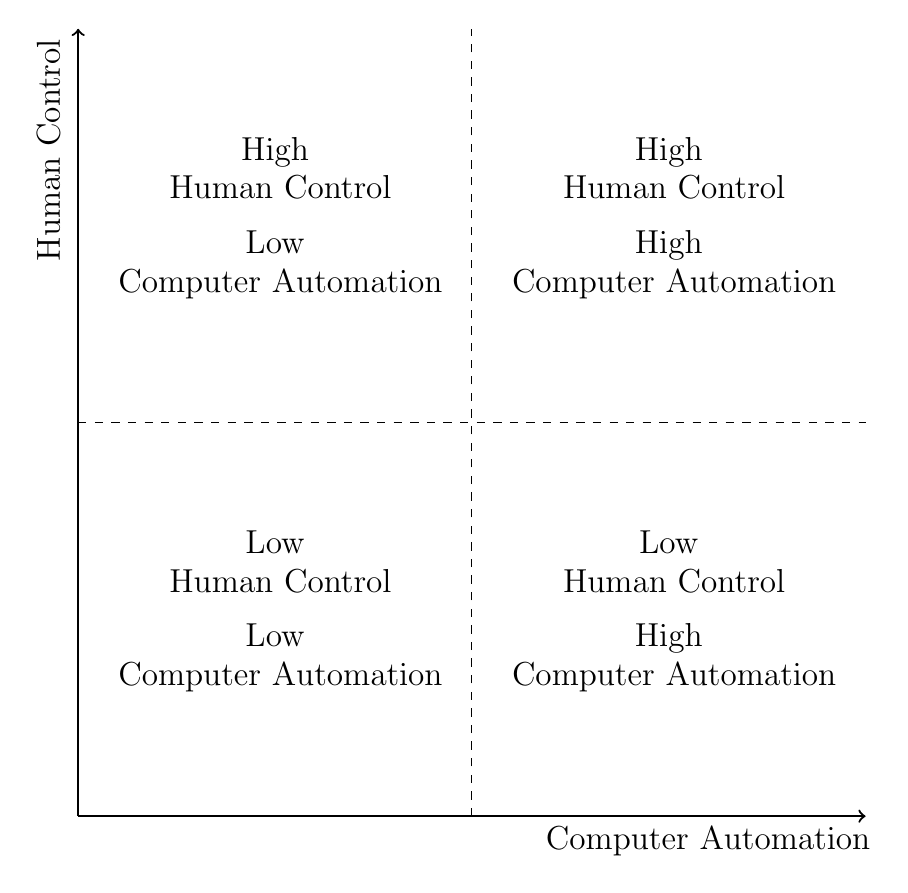
\begin{tikzpicture}
    % Set axis limits
    \draw[->, thick] (0,0) -- (10,0) node[anchor=north, xshift=-2cm, font=\large] {Computer Automation};
    \draw[->, thick] (0,0) -- (0,10) node[anchor=south east, rotate=90, yshift=0.1cm, font=\large] {Human Control};

    \draw[dashed] (0,5) -- (10,5); % Horizontal division
    \draw[dashed] (5,0) -- (5,10); % Vertical division

    \node[align=center, font=\large] at (2.5,2.5) {Low \\ \vspace{0.2cm} Human Control \\ Low \\ \vspace{0.2cm} Computer Automation};
    \node[align=center, font=\large] at (7.5,2.5) {Low \\ \vspace{0.2cm} Human Control \\ High \\ \vspace{0.2cm} Computer Automation};
    \node[align=center, font=\large] at (2.5,7.5) {High \\ \vspace{0.2cm} Human Control \\ Low \\ \vspace{0.2cm} Computer Automation};
    \node[align=center, font=\large] at (7.5,7.5) {High \\ \vspace{0.2cm} Human Control \\ High \\ \vspace{0.2cm} Computer Automation};
\end{tikzpicture}
}
\caption{Two-dimensional HCAI framework of human control and computer automation \cite{shneiderman2022human}.}
\label{fig:HCAI_dimensions}
\end{figure}
  
Building on these principles, \gls{hgml} \cite{gil2019towards} operationalizes   
human-centered design through specific interaction patterns where domain experts   
actively guide and influence the learning process. Rather than treating automation   
as a black box, \gls{hgml} promotes collaborative workflows where experts validate   
intermediate decisions and shape model behaviour. The framework defines concrete   
tasks across three categories: data use (variable selection, variable requirements,   
instance selection), model development (model selection, parameter settings, solution design) and model interpretation (model assessment, model comparison, parameter comparison). These tasks provide a structured framework for evaluating how well an \gls{automl} system supports domain expert involvement. While \gls{hcai} provides high-level design principles for human-AI collaboration, \gls{hgml} translates these into actionable criteria grounded in \gls{ml} workflows, making it particularly suitable for assessing systems that aim to democratize predictive modeling in specialized domains.


\section{Application}  
\label{sec:application}

This section describes the design and implementation of \gls{hamelin}. We first outline the participatory design process that shaped the system, then present the application, its architecture and key components, and finally detail the user interface and workflow that guide \glspl{crp} through the predictive modeling pipeline.

\subsection{Participatory Design Process}
\label{subsec:design_process}
  
The development of \gls{hamelin} followed a collaborative design approach involving 
a \gls{crp} from the Clinical Trials Agency of IDIVAL at Marqu\'es de Valdecilla University Hospital. Rather than 
conducting a formal user study, the process was structured around ongoing 
collaboration: while the data science team held weekly internal meetings to review progress and integrate feedback, the \gls{crp} contributed domain expertise and evaluated the evolving interface against real clinical workflows and protocols every three months throughout the development cycle.

The collaboration was grounded in four real clinical protocols provided by the 
\gls{crp} at the outset of the project, covering the three main research designs 
encountered in clinical practice: one patient registry, one observational study and 
two clinical trials. These protocols served as primary design artifacts, directly 
shaping the interface terminology, workflow structure and validation mechanisms. In 
addition, a real dataset from an observational study was provided to enable functional 
testing of the application under realistic clinical data conditions. The four protocols are described below:

\begin{itemize}
    \item \textbf{COVID-19 Registry}: A multicenter patient registry documenting clinical characteristics, treatments and outcomes of COVID-19 patients. The registry collected demographic variables (age, sex, etc.), comorbidities (hypertension, diabetes, cardiovascular disease), clinical variables (symptoms, laboratory values), treatments (antivirals, corticosteroids, oxygen therapy) and outcomes (hospital discharge, \gls{icu} admission, death).
    
    \item \textbf{Pressure Injuries Study (UPS)}: An observational study investigating the incidence and risk factors of pressure injuries in neurosurgery patients undergoing procedures longer than 3 hours. The protocol specified variables related to patient characteristics (age, sex, BMI, Braden scale score), intraoperative factors (surgical duration, patient positioning, use of pressure-relief surfaces, intraoperative temperature) and postoperative outcomes (presence/absence of pressure injuries, injury severity).
    
    \item \textbf{COLCHI-COVID} (Nº EudraCT: 2020-001603-16): A randomized, double-blind, placebo-controlled clinical trial evaluating the efficacy and safety of colchicine in hospitalized COVID-19 patients \cite{estebanez2021effectiveness}. The protocol defined primary endpoints (clinical improvement at day 14), secondary endpoints (mortality, \gls{icu} admission, adverse events) and detailed inclusion/exclusion criteria (age $\geq$ 18 years, confirmed COVID-19, no contraindications to colchicine).
    
    \item \textbf{VACAB-2022} (Nº EudraCT: 2022-004192-16): A randomized clinical trial evaluating the efficacy of mucosal bacterial vaccines (autovaccines) compared to suppressive antibiotic therapy in patients with hip or knee prosthesis infections. The protocol defined primary endpoints (infection recurrence at 12 months), secondary endpoints (quality of life, adverse events) and inclusion/exclusion criteria (confirmed prosthesis infection, no immunosuppression, no allergy to vaccine components).
\end{itemize}

Each protocol type imposes distinct requirements on the modeling pipeline. Patient registries require flexible variable selection and long-term outcome modeling, with no predefined intervention structure. Observational studies demand careful handling of confounding variables and exposure-outcome relationships. Clinical trials introduce the most complex constraints: explicit inclusion/exclusion criteria defining the study population, temporal phases separating data collection points and endpoint hierarchies distinguishing primary efficacy outcomes from secondary safety and exploratory measures. \gls{hamelin} was designed to accommodate all three study types within a unified interface, ensuring that the modeling pipeline respects the methodological constraints of each design.

The design process was iterative and collaborative. Initial mockups were developed based on the analysis of these clinical protocols and periodically refined through feedback sessions with \glspl{crp}. These mockups served to validate the proposed terminology (for instance, ``primary variable'' in place 
of ``target variable'' and ``criteria'' in place of ``filters''), workflow structure and interaction patterns before full implementation.
  
\subsection{System Overview and Architecture}
\label{subsec:architecture}

\gls{hamelin} is a no-code, protocol-aware \gls{automl} application under development specifically designed to operationalize \gls{hgml} principles for clinical research, enabling \glspl{crp} to build predictive models without programming expertise while incorporating their domain knowledge at every stage of the process.

\begin{figure}[ht]
\centering
\scalebox{0.75}{
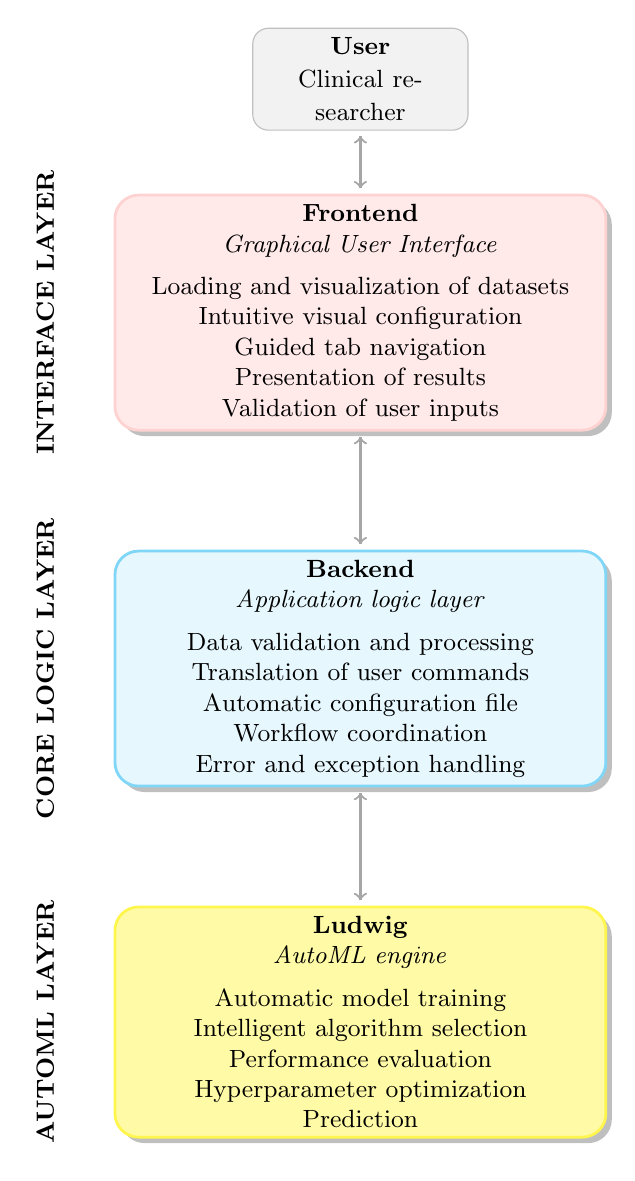
\begin{tikzpicture}[
    node distance=1.5cm,
    box/.style={
        rectangle,
        draw,
        text width=6cm,
        text centered,
        minimum height=2cm,
        rounded corners=0.3cm,
        drop shadow,
        line width=1pt,
        font=\small
    },
    frontend/.style={box, fill=pink!35, draw=pink!70},
    backend/.style={box, fill=cyan!10, draw=cyan!50},
    ludwig/.style={box, fill=yellow!35, draw=yellow!70},
    arrow/.style={->, thick, color=gray!70, line width=0.8pt, shorten >=2pt, shorten <=2pt},
]

\node[frontend] (frontend) at (0,0) {
    \textbf{Frontend}\\
    \textit{Graphical User Interface}\\[1.5mm]
    Loading and visualization of datasets\\
    Intuitive visual configuration\\
    Guided tab navigation\\
    Presentation of results\\
    Validation of user inputs
};

\node[backend, below=1.5cm of frontend.south, anchor=north] (backend) {
    \textbf{Backend}\\
    \textit{Application logic layer}\\[1.5mm]
    Data validation and processing\\
    Translation of user commands\\
    Automatic configuration file\\
    Workflow coordination\\
    Error and exception handling
};

\node[ludwig, below=1.5cm of backend.south, anchor=north] (ludwig) {
    \textbf{Ludwig}\\
    \textit{AutoML engine}\\[1.5mm]
    Automatic model training\\
    Intelligent algorithm selection\\
    Performance evaluation\\
    Hyperparameter optimization\\
    Prediction
};

\draw[arrow] (frontend.south) -- (backend.north);
\draw[arrow] (backend.north) -- (frontend.south);
\draw[arrow] (backend.south) -- (ludwig.north);
\draw[arrow] (ludwig.north) -- (backend.south);

\node[above=0.8cm of frontend.north, 
      rectangle, 
      draw=gray!50, 
      fill=gray!10, 
      text width=2.5cm, 
      text centered,
      rounded corners=0.2cm] (user) {
    \small \textbf{User}\\
    \small Clinical researcher
};
\draw[arrow] (user.south) -- (frontend.north);
\draw[arrow] (frontend.north) -- (user.south);

\node[anchor=center, rotate=90] at ([xshift=-4cm]frontend.center) {\small \textbf{INTERFACE LAYER}};
\node[anchor=center, rotate=90] at ([xshift=-4cm]backend.center) {\small \textbf{CORE LOGIC LAYER}};
\node[anchor=center, rotate=90] at ([xshift=-4cm]ludwig.center) {\small \textbf{AUTOML LAYER}};

\end{tikzpicture}
}
\caption{Layered system architecture of HAMELIN.}
\label{fig:system_architecture}
\end{figure}

\begin{figure*}[h]
\centering
\scalebox{0.8}{
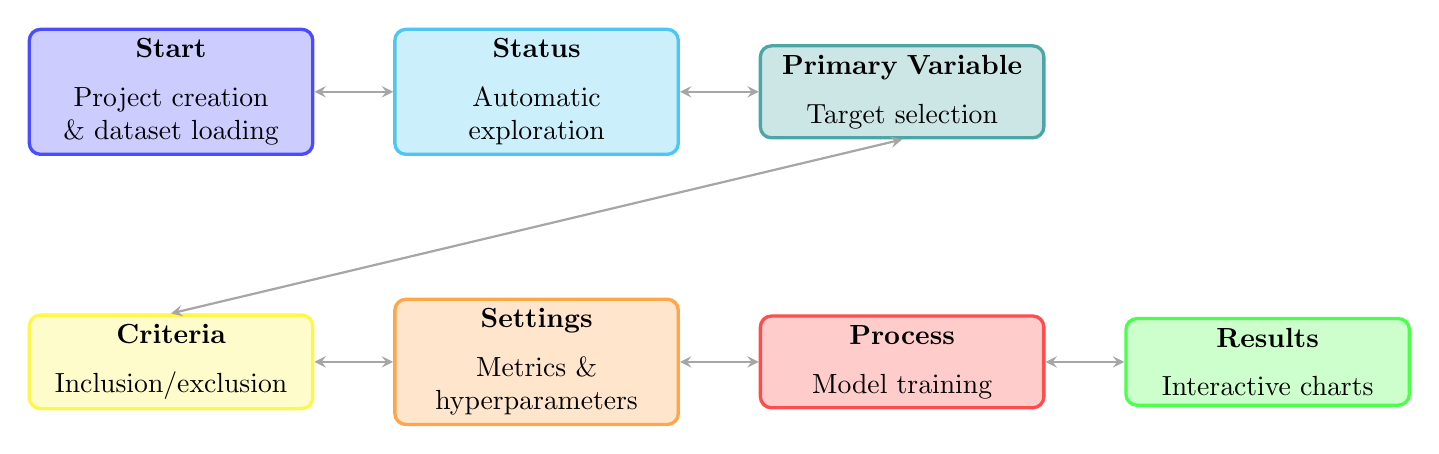
\begin{tikzpicture}[node distance=2.5cm, auto]

    \tikzset{
        mystep/.style={
            rectangle, rounded corners,
            minimum width=3.6cm, minimum height=1cm,
            text centered,
            text width=3.3cm, align=center,
            line width=1.2pt
        },
        arrow/.style={thick,<->,>=stealth, gray!70}
    }

    \node (start)  [mystep, fill=blue!20, draw=blue!70]   
        {\textbf{Start}\\[2mm] Project creation \& dataset loading};

    \node (status) [mystep, fill=cyan!20, draw=cyan!70, right=1.0cm of start] 
        {\textbf{Status}\\[2mm] Automatic exploration};

    \node (primary)[mystep, fill=teal!20, draw=teal!70, right=1.0cm of status] 
        {\textbf{Primary Variable}\\[2mm] Target selection};

    \node (criteria) [mystep, fill=yellow!20, draw=yellow!70, below=2cm of start] 
        {\textbf{Criteria}\\[2mm] Inclusion/exclusion};

    \node (settings) [mystep, fill=orange!20, draw=orange!70, right=1.0cm of criteria] 
        {\textbf{Settings}\\[2mm] Metrics \&\\ hyperparameters};

    \node (process)  [mystep, fill=red!20, draw=red!70, right=1.0cm of settings] 
        {\textbf{Process}\\[2mm] Model training};

    \node (results)  [mystep, fill=green!20, draw=green!70, right=1.0cm of process] 
        {\textbf{Results}\\[2mm] Interactive charts};

    \draw [arrow] (start) -- (status);
    \draw [arrow] (status) -- (primary);
    \draw [arrow] (primary.south) -- (criteria.north);
    \draw [arrow] (criteria) -- (settings);
    \draw [arrow] (settings) -- (process);
    \draw [arrow] (process) -- (results);

\end{tikzpicture}
}
\caption{End-to-end clinical machine learning workflow in HAMELIN.}
\label{fig:workflow}
\end{figure*}

The system architecture follows a three-layer modular design (see Figure~\ref{fig:system_architecture}). The interface layer provides a graphical environment for dataset loading, configuration and visualization. The core logic layer connects the interface to the \gls{automl} engine, handling validation, command translation, configuration file generation, workflow coordination and error handling. The \gls{automl} layer utilizes Ludwig (v0.10.4) to perform automated training, algorithm selection, hyperparameter optimization and evaluation.
  
This modular architecture ensures that the interface logic is separated from the \gls{automl} engine. In principle, Ludwig could be replaced with another \gls{automl} framework without requiring changes to the interface, although some adaptation of the Core Logic Layer would be necessary.
  
\subsection{User Interface and Workflow}
  
The interface employs a tabbed navigation system that guides users through the entire \gls{ml} pipeline. This design provides clear waypoints while maintaining the analytical context, with each tab representing a distinct phase that follows the logical progression typically found in clinical research protocols. A key feature of \gls{hgml} is the ability to refine the model iteratively based on initial results. The \gls{hamelin} interface supports this through a reconfiguration mechanism that allows users to revisit earlier steps and modify their choices based on emerging insights. After reviewing results, users can return to previous tabs to adjust the target variable, refine inclusion/exclusion criteria, select alternative missing data strategies, modify hyperparameter search spaces, or choose different evaluation metrics. Each modification triggers a model re-training cycle with updated results, enabling \glspl{crp} to explore the modeling space systematically, guided by clinical intuition and domain knowledge.



The proposed workflow consists of seven sequential stages (see Figure~\ref{fig:workflow}). The process initiates with project initialization and dataset loading, followed by automated exploratory data analysis to generate descriptive statistics, assess missing data patterns and identify outcome variables. Subsequently, users specify the primary variable, with the system automatically determining the task type (classification or regression). Data filtering is performed through the definition of inclusion and exclusion criteria via a structured interface. The configuration stage encompasses the specification of evaluation metrics, missing data imputation strategies and hyperparameter ranges. Model training is executed with progress tracking, and performance evaluation is presented through comprehensive visualizations including performance metrics, graphical representations and confusion matrices for classification tasks (see Figure~\ref{fig:tab-based_interface}). This iterative refinement process proves particularly valuable in clinical scenarios: for instance, if initial results reveal low sensitivity in detecting at-risk patients, a \gls{crp} might return to the Settings tab to adjust the evaluation metric; alternatively, if feature importance analysis identifies a critical variable with substantial missing data, the imputation strategy can be reconsidered to improve model performance.

\begin{figure*}[ht]  
    \centering  
    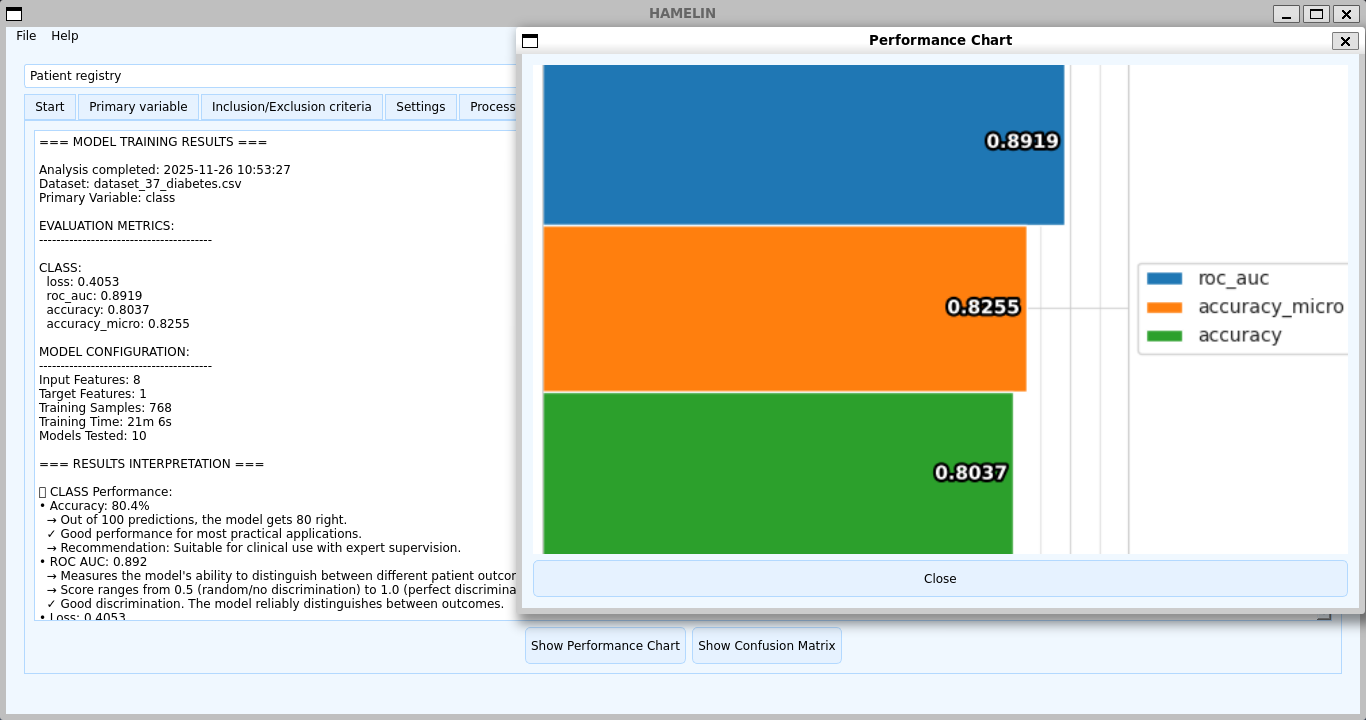
\includegraphics[width=\textwidth]{img/results_tab.png}  
    \caption{Training outcomes and model performance.}  
    \label{fig:tab-based_interface}
\end{figure*}


\section{Alignment with Human-Guided ML}  
\label{sec:hgml_alignment}  
  
To evaluate \gls{hamelin}, we follow the \gls{hgml} criteria \cite{gil2019towards}, which provide a structured framework to assess how domain experts can guide data use, model development and result interpretation in interactive \gls{ml} systems. Applying these criteria highlights both the strengths and limitations of \gls{hamelin} in supporting clinical researchers (see Table \ref{tab:hgml_alignment}).


\begin{table*}[ht]
\caption{Mapping between \gls{hgml} tasks \cite{gil2019towards} and \gls{hamelin} clinical functionalities.}
\label{tab:hgml_alignment}
\centering
\renewcommand{\arraystretch}{1.3}
\begin{tabularx}{\textwidth}{@{}p{0.18\textwidth} p{0.28\textwidth} p{0.32\textwidth} p{0.17\textwidth}@{}}
\toprule
\textbf{Category} & \textbf{HGML task} & \textbf{Where in HAMELIN} & \textbf{Implementation status} \\
\midrule
\multicolumn{4}{l}{\textbf{Data Use}} \\
\midrule
\multirow{5}{*}{\parbox[t]{0.18\textwidth}{Variable Selection}} 
& \parbox[t]{0.28\textwidth}{[VS1] Variable selection (prioritise variables)} & \parbox[t]{0.32\textwidth}{\emph{Primary Variable}, \emph{Settings}} & \parbox[t]{0.17\textwidth}{Partially} \\
& \parbox[t]{0.28\textwidth}{[VS2] Create new variables from existing ones} & \parbox[t]{0.32\textwidth}{-- (external preprocessing)} & \parbox[t]{0.17\textwidth}{Not implemented} \\
& \parbox[t]{0.28\textwidth}{[VS3] Change temporal / spatial framing of variables} & \parbox[t]{0.32\textwidth}{\emph{Criteria}; protocol phases} & \parbox[t]{0.17\textwidth}{Partially} \\
& \parbox[t]{0.28\textwidth}{[VS4] Impute missing values using other variables} & \parbox[t]{0.32\textwidth}{\emph{Settings}} & \parbox[t]{0.17\textwidth}{Fully} \\
& \parbox[t]{0.28\textwidth}{[VS5] Augment data using new sources} & \parbox[t]{0.32\textwidth}{--} & \parbox[t]{0.17\textwidth}{Not implemented} \\
\cmidrule(lr){1-4}
\parbox[t]{0.18\textwidth}{Variable Requirements} 
& \parbox[t]{0.28\textwidth}{[VR1] Require inclusion / exclusion of variables} & \parbox[t]{0.32\textwidth}{\emph{Criteria}} & \parbox[t]{0.17\textwidth}{Fully} \\
\cmidrule(lr){1-4}
\multirow{4}{*}{\parbox[t]{0.18\textwidth}{Instance Selection}} 
& \parbox[t]{0.28\textwidth}{[IS1] Select instances to label / annotate} & \parbox[t]{0.32\textwidth}{--} & \parbox[t]{0.17\textwidth}{Not implemented} \\
& \parbox[t]{0.28\textwidth}{[IS2] Select subpopulation of instances} & \parbox[t]{0.32\textwidth}{\emph{Criteria}} & \parbox[t]{0.17\textwidth}{Fully} \\
& \parbox[t]{0.28\textwidth}{[IS3] Remove specific instances} & \parbox[t]{0.32\textwidth}{\emph{Criteria}} & \parbox[t]{0.17\textwidth}{Fully} \\
& \parbox[t]{0.28\textwidth}{[IS4] Define train/test split and cross-validation} & \parbox[t]{0.32\textwidth}{--} & \parbox[t]{0.17\textwidth}{Not implemented} \\
\midrule
\multicolumn{4}{l}{\textbf{Model Development}} \\
\midrule
\multirow{2}{*}{\parbox[t]{0.18\textwidth}{Model Selection}} 
& \parbox[t]{0.28\textwidth}{[MS1] Request a specific type of model} & \parbox[t]{0.32\textwidth}{\emph{AutoML Layer} (Ludwig)} & \parbox[t]{0.17\textwidth}{Partially} \\
& \parbox[t]{0.28\textwidth}{[MS2] Replace the model in a prior solution} & \parbox[t]{0.32\textwidth}{--} & \parbox[t]{0.17\textwidth}{Not implemented} \\
\cmidrule(lr){1-4}
\parbox[t]{0.18\textwidth}{Parameter Settings} 
& \parbox[t]{0.28\textwidth}{[PT1] Request specific parameter values} & \parbox[t]{0.32\textwidth}{\emph{Settings}, Hyperparameter search (Ludwig)} & \parbox[t]{0.17\textwidth}{Partially} \\
\cmidrule(lr){1-4}
\multirow{2}{*}{\parbox[t]{0.18\textwidth}{Solution Design}} 
& \parbox[t]{0.28\textwidth}{[SD1] Request specific data-preparation steps} & \parbox[t]{0.32\textwidth}{\emph{Settings}} & \parbox[t]{0.17\textwidth}{Fully} \\
& \parbox[t]{0.28\textwidth}{[SD2] Replace a data-preparation step} & \parbox[t]{0.32\textwidth}{\emph{Settings}} & \parbox[t]{0.17\textwidth}{Fully} \\
\midrule
\multicolumn{4}{l}{\textbf{Model Interpretation}} \\
\midrule
\multirow{2}{*}{\parbox[t]{0.18\textwidth}{Model Assessment}} 
& \parbox[t]{0.28\textwidth}{[QC1] Request quantities of interest / metrics} & \parbox[t]{0.32\textwidth}{\emph{Results}} & \parbox[t]{0.17\textwidth}{Fully} \\
& \parbox[t]{0.28\textwidth}{[QC2] Request intermediate results} & \parbox[t]{0.32\textwidth}{--} & \parbox[t]{0.17\textwidth}{Not implemented} \\
\cmidrule(lr){1-4}
\multirow{5}{*}{\parbox[t]{0.18\textwidth}{Model Comparison}} 
& \parbox[t]{0.28\textwidth}{[MC1] Compare solutions with different model types} & \parbox[t]{0.32\textwidth}{--} & \parbox[t]{0.17\textwidth}{Not implemented} \\
& \parbox[t]{0.28\textwidth}{[MC2] Compare solutions on different subsets of instances} & \parbox[t]{0.32\textwidth}{--} & \parbox[t]{0.17\textwidth}{Not implemented} \\
& \parbox[t]{0.28\textwidth}{[MC3] Compare solutions with same model but different data prep} & \parbox[t]{0.32\textwidth}{--} & \parbox[t]{0.17\textwidth}{Not implemented} \\
& \parbox[t]{0.28\textwidth}{[MC4] Compare solutions with same model but different parameters} & \parbox[t]{0.32\textwidth}{--} & \parbox[t]{0.17\textwidth}{Not implemented} \\
& \parbox[t]{0.28\textwidth}{[MC5] Compare two models with all other steps equal} & \parbox[t]{0.32\textwidth}{--} & \parbox[t]{0.17\textwidth}{Not implemented} \\
\cmidrule(lr){1-4}
\parbox[t]{0.18\textwidth}{Parameter Comparison} 
& \parbox[t]{0.28\textwidth}{[PC1] Several solutions with same model and varying parameter ranges} & \parbox[t]{0.32\textwidth}{--} & \parbox[t]{0.17\textwidth}{Not implemented} \\
\bottomrule
\end{tabularx}
\end{table*}

  
\subsection{Data Use}  
  
\gls{hamelin} offers strong support for data-centric tasks. Clinicians can select variables [VS1] through the Primary Variable and Settings tabs, although without yet prioritizing variables based on clinical hypotheses. They can change temporal framing of variables [VS3] through the Criteria tab by defining protocol phases, though this feature is still under development. They can impute missing values [VS4] using Ludwig's comprehensive set of strategies, exposed in the Settings tab with clinical explanations. They can require inclusion or exclusion of variables [VR1] through the Criteria tab, which provides an intuitive rule builder for specifying complex inclusion/exclusion logic. They can select subpopulations of instances [IS2] and remove specific instances [IS3] through the same Criteria tab.
  
However, some data-centric tasks are not yet supported. Users cannot create new variables from existing ones [VS2] within the interface; this must be done through external preprocessing. They cannot augment data using new sources [VS5]. They cannot select instances to label or annotate [IS1], as \gls{hamelin} assumes that all data are already labeled. And they cannot define train/test split and cross-validation [IS4] through the Settings tab, choosing from k-fold, leave-one-out, or temporal split strategies.
  
\subsection{Model Development}
  
Regarding model development, \gls{hamelin} relies on the underlying \gls{automl} backend (Ludwig) for model selection and hyperparameter tuning. Users have high-level control over preprocessing and training options but not detailed control over model choices. Ludwig automatically selects the model family [MS1] based on data characteristics and task type, but users cannot explicitly request a specific model type (e.g., ``use only logistic regression''). Users cannot replace the model in a prior solution [MS2] or compare solutions with different model types [MC1] within the interface.
  
Users can request specific parameter values [PT1] through the Settings tab by defining custom hyperparameter search spaces, though this requires some familiarity with hyperparameters. Users can request specific data-preparation steps [SD1] and replace data-preparation steps [SD2] through the Settings tab by choosing missing data strategies.
  
\subsection{Model Interpretation}
  
In model interpretation, domain metrics are available. Users can request quantities of interest and metrics [QC1] through the Results tab, which presents accuracy, loss, area under the curve receiver operating characteristic (AUC\_ROC), mean absolute error (MAE), root mean squared error (RMSE). However, users cannot request intermediate results [QC2], such as the performance of models evaluated during hyperparameter search.
  
Systematic comparison of alternative solutions is a significant limitation. Users cannot compare solutions with different model types [MC1], on different subsets of instances [MC2], with the same model but different data preparation [MC3], with the same model but different parameters [MC4], or two models with all other steps equal [MC5]. They cannot generate several solutions with the same model and varying parameter ranges [PC1]. These comparison tasks would require the system to maintain a history of all models trained and to provide interfaces for selecting and comparing them, which is not currently implemented.


\section{Discussion}  
\label{sec:discussion}

The development of \gls{hamelin} demonstrates that protocol-aware \gls{automl} systems can help bridge the gap between advanced \gls{ml} techniques and their practical adoption in clinical research. By involving \glspl{crp} throughout the design process and grounding the interface in real clinical protocols, the system aligns more closely with established clinical research practices than generic \gls{automl} tools.
  
This alignment is the result of several design decisions. First, the use of clinical terminology (e.g., ``primary variable'' instead of ``target variable'', ``criteria'' instead of ``filters'') improves accessibility and reduces cognitive friction for \glspl{crp}. Second, the tab-based workflow reflects the logical sequence of a clinical study, formulating the research question, preparing data, defining the study population, configuring the analysis, executing the models and interpreting the results, providing a familiar and intuitive structure. Third, explicit support for inclusion and exclusion criteria addresses a critical gap in existing \gls{automl} systems and ensures that models are trained on valid populations. Finally, exposing Ludwig's missing data strategies with clinically grounded explanations enables users to make informed decisions about a complex preprocessing step.  
  
Despite these strengths, the evaluation against \gls{hgml} criteria reveals  
important limitations. While \gls{hamelin} offers strong support for data-centric  
tasks, it provides limited functionality for model-centric and comparison tasks.  
Users cannot explicitly choose model families, compare alternative models, or  
systematically explore different modeling strategies. These limitations reflect a  
broader tension in \gls{automl} system design between automation and user control.  
In its current form, \gls{hamelin} prioritizes automation in model selection and  
hyperparameter tuning, delegating these decisions to Ludwig.

Future research should investigate how to introduce greater user control over modeling decisions without overwhelming \glspl{crp} with technical complexity. A promising direction is the integration of large language models (LLMs) as conversational interfaces \cite{miguel2025integrating}, where users interact with the \gls{ml} pipeline through natural language prompts. In addition, the current system lacks support for feature engineering within the interface. Clinical researchers often need to define derived variables (e.g., body mass index from weight and height, interaction terms, or nonlinear transformations) based on domain knowledge. At present, such transformations require external preprocessing, disrupting the workflow and requiring programming skills. Future versions of \gls{hamelin} should therefore incorporate an interface for feature engineering that allows users to specify transformations using domain-meaningful concepts.

Finally, the collaborative design process described in this work, while grounded in 
real clinical protocols and sustained engagement with a \gls{crp}, does not 
constitute a formal usability evaluation. The evidence gathered is qualitative and 
reflects the perspective of a single domain expert. A structured user study involving a broader and more diverse sample of \glspl{crp} is planned as future work to formally assess the usability, learnability and practical effectiveness of \gls{hamelin} in real-world clinical research settings.


\section{Conclusions}  
\label{sec:conclusions}

This work presents \gls{hamelin}, a protocol-aware \gls{automl} tool that enables clinical researchers without programming expertise to build predictive models while partially satisfying the criteria for \gls{hgml}. By embedding protocol-aware constraints, the system ensures that predictive models respect temporal structures, endpoint hierarchies and inclusion/exclusion criteria, across patient registries, observational studies and clinical trials. This design enhances clinical validity and coherence, distinguishing the approach from existing domain-agnostic \gls{automl} platforms that treat clinical datasets as generic matrices.

The evaluation demonstrates strong support for data-centric operations, including variable selection, subpopulation definition and inclusion/exclusion logic. However, model-centric tasks, such as explicit model family selection, hyperparameter specification and systematic comparison of alternative solutions, remain partially constrained. Ongoing development aims to extend interactive control over these stages and incorporate advanced features such as feature engineering, provenance tracking and multi-source data integration, moving the system toward full \gls{hgml} compliance where domain expertise can guide all aspects of the modeling process.



\bibliographystyle{IEEEtran}
\bibliography{bibliography.bib}

\end{document}
